\documentclass{article}
\usepackage{tikz}
\usepackage{ifthen}
\usetikzlibrary{arrows}

% type, redundancy, required, lambda 
\newcommand{\modelgraphlabel}[4]{$#1$ \\ $r=#2$ \\ $\nu=#3$ \\ $\lambda=#4$}

\begin{document}
% Cloud Model 
% draw - outline, fill - color!alpha, align - allows for manual linebreak
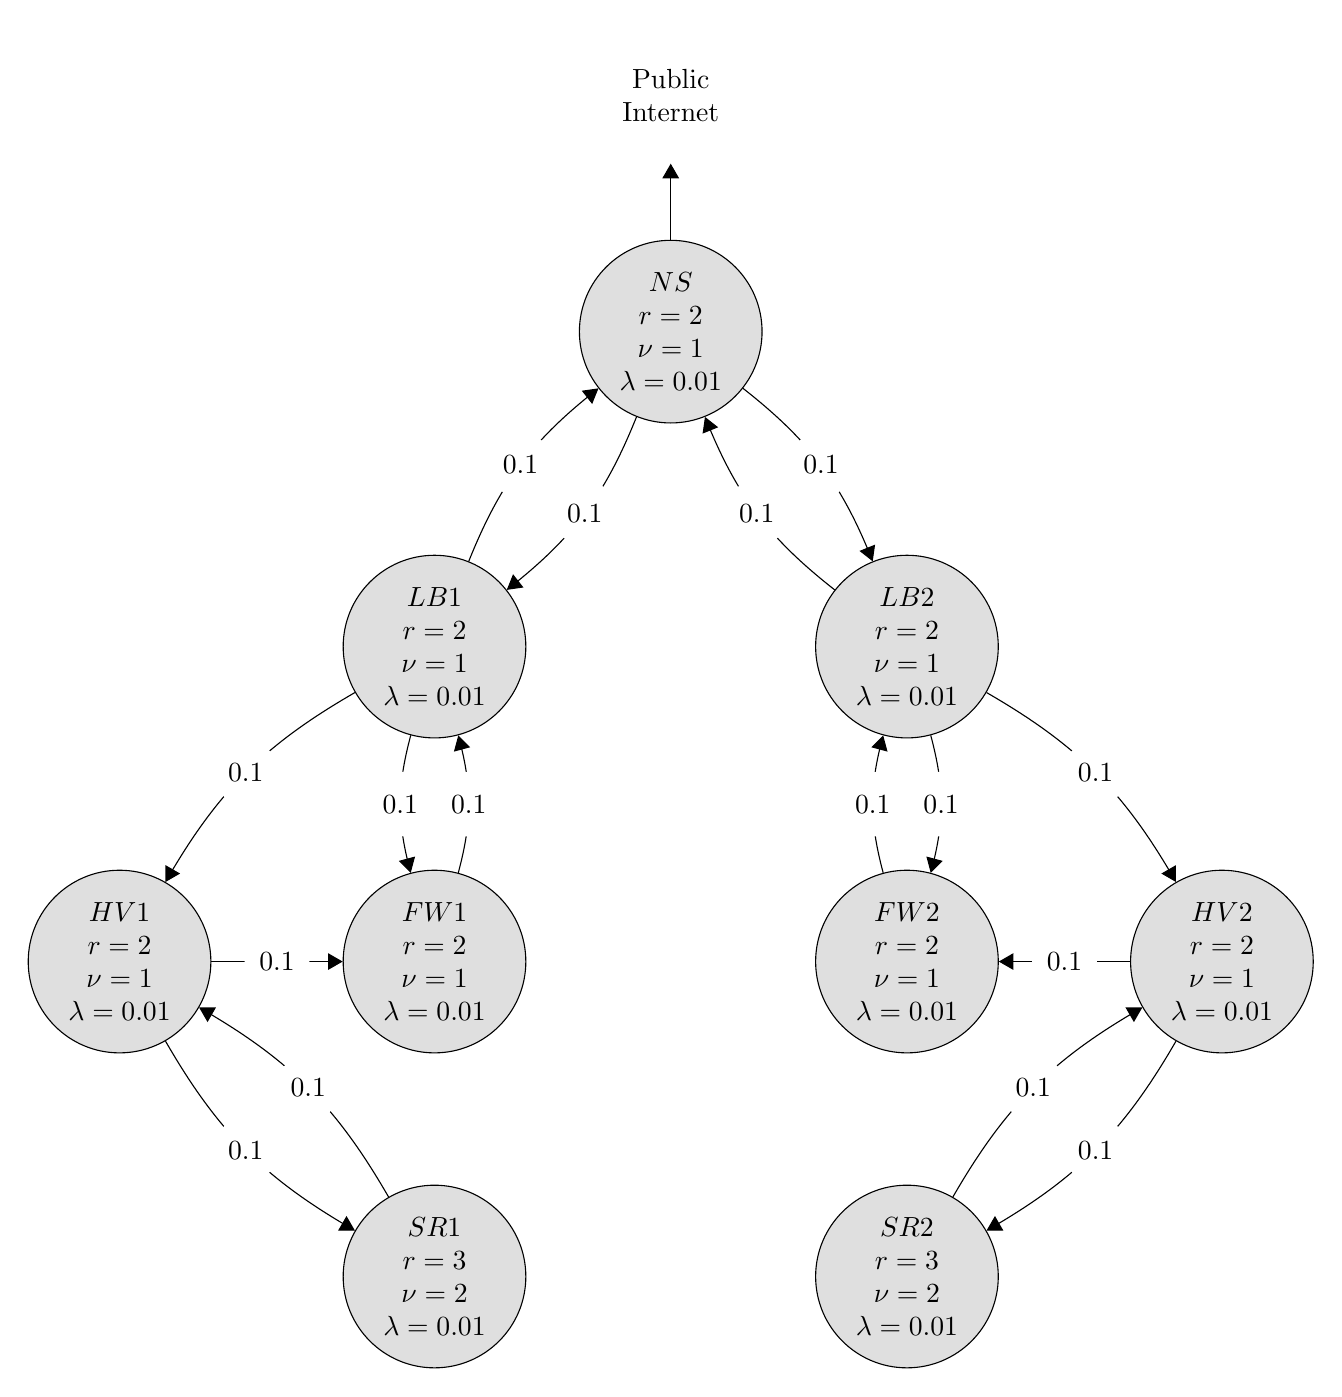
\begin{tikzpicture}[scale = 1, auto = center, every node/.style = {circle, draw = black, fill = gray!25}, bend angle = 90]

	\node (NS)  at ( 3, 16) [align = center] {\modelgraphlabel{NS}  {2}{1} {0.01} };
	\node (LB1) at ( 0, 12) [align = center] {\modelgraphlabel{LB1} {2}{1} {0.01} };
	\node (LB2) at ( 6, 12) [align = center] {\modelgraphlabel{LB2} {2}{1} {0.01} };
	\node (FW1) at ( 0,  8) [align = center] {\modelgraphlabel{FW1} {2}{1} {0.01} };
	\node (FW2) at ( 6,  8) [align = center] {\modelgraphlabel{FW2} {2}{1} {0.01} };
	\node (HV1) at ( -4,  8) [align = center] {\modelgraphlabel{HV1} {2}{1} {0.01} };
	\node (HV2) at ( 10,  8) [align = center] {\modelgraphlabel{HV2} {2}{1} {0.01} };
	\node (SR1) at ( 0,  4) [align = center] {\modelgraphlabel{SR1} {3}{2} {0.01} };
	\node (SR2) at ( 6,  4) [align = center] {\modelgraphlabel{SR2} {3}{2} {0.01} };
	\node (PB) at ( 3, 19) [align = center, fill=none, draw=none] {Public\\Internet};

    \foreach \from/\phy/\to in {NS/0.1/LB1, NS/0.1/LB2, LB1/0.1/NS, LB2/0.1/NS, 
    LB2/0.1/FW2, FW2/0.1/LB2, LB2/0.1/HV2, SR2/0.1/HV2, HV2/0.1/SR2}
    	\path (\from) edge [-triangle 60, bend left = 15] node[fill=white, draw=none] {\phy} (\to);
    \foreach \from/\phy/\to in {LB1/0.1/FW1, FW1/0.1/LB1, LB1/0.1/HV1, SR1/0.1/HV1, HV1/0.1/SR1}
    	\path (\from) edge [-triangle 60, bend right = 15] node[fill=white, draw=none] {\phy} (\to);
    \foreach \from/\phy/\to in {HV1/0.1/FW1,HV2/0.1/FW2}
    	\path (\from) edge [-triangle 60] node[fill=white, draw=none] {\phy} (\to);

    \path (NS) edge [-triangle 60] node[fill=none, draw=none] {}(PB);

\end{tikzpicture}

\end{document}